\chapter{Další metody testování hypotéz}
\begin{example}
	Mějme $X\sim\mathrm{Po}(\lambda),$ tedy $\E X=\lambda$, a~testujme hypotézu \mbox{$\hypothesis{\lambda=1}{\lambda=10}$.} Použijeme-li optimální test
	$\txt{UMP}_{\alpha=0.05}:~\Phiast=\begin{cases}
	1&x\geq4,\\0.5058&x=3,\\0&x\leq2,
	\end{cases}$\\ dostaneme sílu tohoto UMP testu 
	$ \beta=\beta_{\Phiast}(10)=1-0.0065$, tzn., že $\PP(\text{chyby II. druhu})=0.0065 $ je ještě o~řád nižší, než $\PP(\text{chyby I. druhu})=\alpha=0.05$, kterou považujeme za~kritickou (vážnější) chybu. Kritickou chybu tak máme pod~horší kontrolou, než nekritickou chybu.
	\\Pokud v~praxi použijeme \textbf{neoptimální }test $\crossedphi=\begin{cases}
	1&x\geq6,\\0.4516&x=5,\\0&x\leq4,
	\end{cases}$\\
	pro který $\alpha=0.0019$ se~sílou testu $\beta=0.95$, dostaneme test s~lepší kontrolou kritické \mbox{$\PP(\text{chyby I. druhu})=0.0019 $}, při~zachování rozumné velikosti $1-\beta=0.05$ pro~pravděpodobnost nekritické chyby II. druhu. 
	
	Zabývejme se~dále i~dalšími potenciálně neoptimálními testy, jako je například LRT test. 
\end{example}
\section{Test poměrem věrohodností (LRT)}
\begin{define}
	Mějme rodinu $\mathcal{F}=\{f(x,\t):\t\in\Theta\}$ a~testujme obecnou hypotézu\\ $H_0:\t\in\Theta_0~\text{vs.}~H_1:\t\in\Theta_1$ na~zadané hladině významnosti $\alpha\in(0,1)$.
	Zaveďme funkci
	$$ \Lambda(\textbf{x}):=\frac{\sup\limits_{\t\in\Theta_0}L(\t)}{\sup\limits_{\t\in\Theta_0\cup\Theta_1}L(\t)},\quad\text{ kde } L(\t)=f(\textbf{x},\t) $$ je věrohodnostní funkcí testovaného modelu, založenou na~vzorku $\textbf{x}\in\mathcal{X}$ z~náhodného výběru $\X=(X_j)_{j=1}^n~iid~f(x,\t)$. Definujme test tvaru $$\crossedphi_\Lambda(\textbf{x})=\begin{cases}
	1&\textbf{x}\in W_\Lambda\subset\R^n,\\0&\textbf{x}\notin W_\Lambda,
	\end{cases}$$ kde $W_\Lambda=\{ \textbf{x}\in\R^n:~\Lambda(\textbf{x})\leq K~\}$ je taková, že pro~nějakou konstantu $K\in[0,1]$ platí $\beta_{\crossedphi_\Lambda}\big|_{\Theta_{0}}\leq\alpha$, tzn.
	 $$\beta_{W_\Lambda}(\t):=\beta_{\crossedphi_\Lambda}(\t)=\E_\t \crossedphi_\Lambda(\X)=\PP_\t
	\br{\crossedphi_\Lambda(\X)=1}\leq \alpha,~\forall\t\in\Theta_0.$$  Takové $\crossedphi_\Lambda$, pokud existuje, se~nazývá \textbf{LRT test} pro~testování $H_0\times H_1$ na~hladině významnosti $\alpha$, ozn. $\txt{LRT}_\alpha$. $W_\Lambda$ je odpovídající LRT kritická oblast tohoto testu ($\txt{LRT}_\alpha$ CR). Pokud nastal jev 
	$\{ \X\in W_\Lambda	\}$, zamítáme $H_0$, pokud nastává opačný jev, pak $H_0$ nezamítneme.
\end{define}
Jde o~test založený na~limitních vlastnostech statistického modelu, přičemž smysluplnost zavedení tohoto LRT testů vyplývá z~lemmatu, dokázaného v~sekci 2 MLE odhadů, které říká, že pro~$\posl~iid~f(x,\t_0),$ kde $\supp f$ je nezávislý na~$\t$, platí, že  $$\PP_{\t_0}\br{L(\t_0)>L(\t)}\stackrel{n\to+\infty}{\longrightarrow}1,\quad\forall\t\neq\t_0.$$ 
	\begin{enumerate}[a)]
		\item Pokud $H_0$ platí, a~tedy skutečná hodnota parametru $\t_0$ leží jak v~$\Theta_0$, tak v~$\Theta_0\cup\Theta_1$, pak $\Lambda(\textbf{x})=\frac{\sup\limits_{\t\in\Theta_0}L(\t)}{\sup\limits_{\t\in\Theta_0\cup\Theta_1}L(\t)}=1$ s~pravděpodobností $\PP_{\t_0}$ jdoucí k~1 při~$n\to+\infty$.
		\item Pokud $H_0$ neplatí, a~tedy skutečná hodnota parametru $\t_0$ neleží v~$\Theta_0$, ale stále je obsažena ve~$\Theta_0\cup \Theta_1$, pak  $\Lambda(\textbf{x})\leq K<1$ je ostře odraženo od~1 s~pravděpodobností $\PP_{\t_0 }$ jdoucí k~$1$ při~$n\to+\infty$. Právě tak jsme nastavili v~definici $\crossedphi_\Lambda$ kritický obor $W_\Lambda$ pro~přijetí/zamítnutí $H_0$.
	\end{enumerate}
\begin{remark}
	LRT test nemusí být obecně optimální, je založen pouze na~asymptotické vlastnosti a~tedy pro~konečné $n$ nemusí dosahovat uspokojivých kvalit ve~své síle testu $\beta$. Dokonce lze nalézt příklady LRT testů, které mají sílu testu $\beta$ nižší, než zadaná hranice $\alpha$ pro~chybu I. druhu, tzn. chyba II. druhu je velmi častá!
	
	LRT test je v~praxi často využíván pro~svou obecnost $(\t\in\R^k)$, někdy za~cenu složitější implementace při~vyhodnocování funkce $\Lambda(\textbf{x})$ nebo při~řešení distribučního problému rozdělení testovací statistiky $T_\Lambda(\X)$ za~platnosti $H_0$.
\end{remark}

\begin{example}[jednovýběrový t-test: podrobněji v~MASC]
	Mějme $X_1,...,X_n~iid~\n{\mu,\sigma^2}$, kde $\sigma^2$ \textbf{neznáme}. Testujeme hypotézu
	\mbox{$\hypothesis{\mu=\mu_0}{\mu\neq \mu_0}$} na~hladině $\alpha$ pro~nějaké vybrané $\mu_0\in\R$ fixní. Pak zde máme
	$$\t=(\mu,\sigma^2),~\Theta_0=\mu_0\times\R^+,~\Theta=\Theta_0\uplus\Theta_1=\R\times\R^+,$$
	$$ \Lambda(\textbf{x})=\frac{\sup L(\mu_0,\sigma^2):\sigma>0}{\sup L(\mu,\sigma^2):\mu\in\R,\sigma>0},$$
	kde $L(\mu,\sigma^2)$ je věrohodnostní funkce odpovídajícího systému $\mathcal{F}_n=\left\{ \prod\limits_{j=1}^n f_{X_j} \right\}$. Z~teorie ML odhadů vyplývá, že supréma $L$ se~nabývá právě v~bodech maximálně věrohodných odhadů v~čitateli i~jmenovateli, tzn.
	\[
	\begin{split}
	\widehat{\sigma}_{0n}^2&=\argmax\limits_{\sigma^2}L(\mu_0,\sigma^2)=\frac{1}{n}\sumjn (X_j-\mu_0)^2\text{ a~}\\
	(\widehat{\mu}_{n},\widehat{\sigma}_{n}^2)&=\argmax\limits_{(\mu,\sigma^2)}L(\mu,\sigma^2)=\Br{\Oxn,\frac{1}{n}\sumjn (X_j-\Oxn)^2}.
	\end{split}
	\]
	Dosazením do~$\Lambda(\textbf{x})$ a~upravením nerovnosti $\Lambda(\textbf{x})<K$ získáme $\txt{LRT~CR}$ ve~tvaru\\ \mbox{$W_\Lambda=\left\{ \textbf{x}\in\R^n:\frac{\sqrt{n}\abs{\oxn-\mu}}{s_n}\geq K' \right\},$} kde $s_n=\frac{n}{n-1}\widehat{\sigma}_n$ je výběrová směrodatná odchylka. Zavedením $\txt{LRT}$ testovací statistiky $T_\Lambda(\X)=\frac{\sqrt{n}(\Oxn-\mu)}{s_n}\sim t(n-1)$ určíme $K'=t_{1-\frac{\alpha}{2}}(n-1)$-kvantil Studentova rozdělení s~$(n-1)$ stupni volnosti, aby bylo naplněno, že pro~$\forall\sigma^2>0$ 
	$$ \beta_{W_\Lambda}(\mu_0,\sigma^2)=\PP_{H_0}(\text{chyby I. druhu})=\PP_{H_0}(T_\Lambda(\X)\geq t_{1-\frac{\alpha}{2}}(n-1))=\alpha. $$  Upozornění: v~případě tohoto obecně neoptimálního $\txt{LRT}$ testu je velmi žádoucí výpočet, resp. aproximace, síly testu v~okolí $H_{\mu_0}^+$ (pravé okolí bodu $\mu_0$). 
\end{example}

\section{Analýza variance (ANOVA)}
Analýza rozptylu (\textit{analysis of variance, ANOVA}) je metoda, která umožňuje zjistit, jestli má na~Gaussovskou náhodnou veličinu vliv některý ze~znaků u~jednotlivých jedinců, např. zda na~plat zaměstnanců má vliv dosažené vzdělání, pohlaví, věk apod.

Mějme nezávislé náhodné výběry $X_{i1},...,X_{in_i}\sim\n{\mu_i,\sigma^2},~i\in I,~N=\sum_{i=1}^{I}n_i$. Potom sdružená hustota z~$\mathcal{F}_N$ je tvaru
$$ f(\textbf{x}|\mu_1,...,\mu_I,\sigma^2)=(2\pi\sigma^2)^{-\frac{N}{2}}\exp\left\{ -\frac{1}{2\sigma^2}\sum_{i=1}^{I}\sum_{j=1}^{n_i}(x_{ij}-\mu_i)^2 \right\}. $$
Testujeme hypotézu
$$ \hypothesiswide{\mu_1=\mu_2=...=\mu_I(=\mu)}{\text{alespoň jedna nerovnost}} $$
na hladině $\alpha\in(0,1)$ za~dodatečného předpokladu $\sigma_1^2=...=\sigma_I^2=\sigma^2$ neznámé, tzn. předpokládáme homogenitu rozptylů jednotlivých testovaných podskupin $i\in I$.

\subsection*{Odvození ANOVA $\txt{LRT}_\alpha$ testu}
Mějme
$$ \Lambda(\textbf{x})=\frac{\sup\{ f(\textbf{x}|\mu,\mu,...,\mu,\sigma^2):\mu\in\R,\sigma^2>0 \}}{\sup\{ f(\textbf{x}|\mu_1,\mu_2,...,\mu_I,\sigma^2):\mu_i\in\R,\sigma^2>0 \}}. $$
Při řešení extrémů prostřednictvím diferenciálního počtu $\partial_r f=0$ v~čitateli získáme $2$ rovnice a~ve~jmenovateli $I+1$ rovnic, které vyřešíme a~příslušné hodnoty maximálně věrohodných odhadů $\widehat{\mu},\widehat{\sigma}^2$, resp. $\widehat{\mu}_i,\widehat{\sigma}^2,~i\in I$, zpětně dosadíme do~$\Lambda(\textbf{x})$. Dále potom nalezneme tvar LRT kritické oblasti $W_\Lambda=\left\{ \textbf{x}:\Lambda(\textbf{x})\leq K~\right\}$, kdy platí
$$ \Lambda(\textbf{x})\leq K\quad\Leftrightarrow\quad\mathcal{F}_\Lambda(\textbf{x})=\frac{(N-I)S_A}{(I-1)S_e}\geq C, $$ kde $$
S_A=\sum_{i=1}^{I}n_i(\overline{x}_i-\overline{\overline{x}})^2,\qquad S_e=\sum_{i=1}^{I}\sum_{j=1}^{n_i}(x_{ij}-\overline{x}_i)^2,\qquad \overline{x}_i=\frac{1}{n_i}\sum_{j=1}^{n_i}x_{ij},\quad\text{a}\quad \overline{\overline{x}}=\frac{1}{N}\sum_{i=1}^{I}\sum_{j=1}^{n_i}x_{ij}.
$$

\begin{example}
	Distribuční problém tohoto LRT testu ANOVA spočívá v~odvození rozdělení testovací statistiky $\mathcal{F}_\Lambda(\textbf{x})$ za~předpokladu platnosti $H_0:\mu_1=...=\mu_I=\mu$. Postupujeme následovně:
	\[
	\begin{split}
	\sm{i=1}{I}\sm{j=1}{n_i}X_{ij}^2&=\sm{i=1}{I}\sm{j=1}{n_i}(X_{ij}-\Ox{i}+\Ox{i})^2=\sm{i=1}{I}\sm{j=1}{n_i}(X_{ij}-\Ox{i})^2+\underbrace{2\sm{i=1}{I}\sm{j=1}{n_i}\Ox{i}(X_{ij}-\Ox{i})}_{0}+\sm{i=1}{I}n_i\Ox{i}^2=\\&=\underbrace{\sm{i=1}{I}\sm{j=1}{n_i}(X_{ij}-\Ox{i})^2}_{Q_1=S_e}+\sm{i=1}{I}n_i(\Ox{i}-\overline{\overline{X}}+\overline{\overline{X}})^2=\\&=S_e+\underbrace{\sm{i=1}{I}n_i(\Ox{i}-\overline{\overline{X}})^2}_{Q_2=S_A}+\underbrace{2\sm{i=1}{I}n_i\overline{\overline{X}}(\Ox{i}-\overline{\overline{X}})}_{0}+\underbrace{\sm{i=1}{I}\overline{\overline{X}}^2n_i}_{N\cdot \overline{\overline{X}}^2=: Q_3}=S_e+S_A+Q_3=\sm{i=1}{3}Q_i,
	\end{split}
	\]
což je součet tří kvadratických forem. Dá se~ukázat (viz lineární algebra), že součet hodností těchto tří kvadratických forem dává plnou dimenzi úlohy $N$,
	$$\sum_{i=1}^{3}h(Q_i)=h(S_e)+h(S_A)+h(Q_3)=(N-I)+(I-1)+1=N.$$ Z~Cochranovy věty pak vyplývá, že $Q_i$ jsou \textbf{nezávislé} a~\mbox{$Q_i(\X)\sim\chi^2\br{h(Q_i)}$}, důsledkem čehož
	$$ \mathcal{F}_\Lambda(\textbf{x})\big|_{H_0}=\frac{S_A/(I-1)}{S_e/(N-I)}\sim \frac{\chi^2{(I-1)}/(I-1)}{\chi^2{(N-I)}/(N-I)}\sim \FF(I-1,N-I),$$
tedy $\mathcal{F}_\Lambda(\textbf{x})$ má za~platnosti $H_0$ Fisherovo rozdělení s~$(I-1)$ a~$(N-I)$ stupni volnosti.
\end{example}

Nyní hledáme konstantu $C$ tak, aby platilo $\PP_{H_0}\br{\mathcal{F}_\Lambda(\X)\geq C}=\alpha$, což vede na~LRT kritický obor $W_\Lambda=\left\{ \textbf{x}:\mathcal{F}_\Lambda(\textbf{x})\geq \FF_{1-\alpha} (I-1,N-I) \right\}$, kde 
$\FF_{1-\alpha}$ značí $(1-\alpha)$-kvantil příslušného Fisherova rozdělení $\FF$. Skončí-li experiment v~tomto kritickém oboru, pak zamítáme $H_0$.

\section{Odůvodnitelné testy (RT)}
Doteď jsme při~TSH postupovali podle následujícího schématu:\begin{itemize}
	\item stanovení principu testu (UMP, UMPU, LRT,...), nastavení $\alpha\in(0,1)$,
	\item odvození $\crossedphi=1/\gamma/0$, tzn. nalezení $W_\alpha$ ve~vhodném tvaru $\{ T(\X)\gtreqless K_\alpha \}$,
	\item řešení distribučního problému, tj. nalezení rozdělení testovací statistiky $T(\X)\big|_{H_0}\sim\FF_T$ při~platnosti $H_0$,
	\item určení $K_\alpha$ z~podmínky $\PP\br{T(\X)\gtreqless K_\alpha}\leq \alpha$ při~platnosti $H_0$, tzn. $\silofunkce{0}\leq \alpha$,
	\item výpočet síly $\beta$ nebo silofunkce testu $\silofunkce{1}$, tzn. $\PP\br{T(\X)\gtreqless K_\alpha}$ při~platnosti $H_1$.
\end{itemize}
Odůvodnitelné testy (\textit{reasonable}, RT) \textbf{přímo} využívají nějakou vhodnou ("uhádnutou") statistiku $T(\X)$, pro~kterou lze nalézt její rozdělení $T(\X)|H_0\sim\FF_T$ takové, že $\FF_T$ nezávisí na~neznámých testovaných parametrech $\t$ . Poté navrhneme logicky vhodný (zdůvodnitelný) test $\crossedphi_\alpha$, např. ve~tvaru $W_\alpha=\left\{ T(\X)\gtreqless K_\alpha \right\}$, doladíme hodnotu $K_\alpha$ a~nakonec spočteme silofunkci testu, což je v~tomto případě velmi žádoucí, pokud to lze. Pokud ne, prověřujeme sílu odvozeného testu numerickou simulací Monte-Carlo nebo použijeme různé aproximace (např. pomocí CLT). Příklady RT testů si ukážeme v~následující sekci!

\section{Dvouvýběrové testy ($2\times\mathcal{N}_1$)}
\textbf{Dvouvýběrový nepárový t-test} porovnává střední hodnoty dvou Gaussovských výběrů. Příkladem toho může být třeba střední hodnota tlaku krve u~kuřáků a~nekuřáků, atp. 

\begin{example}[Dvouvýběrový t-test]\label{dvouvyber} Uvažujme dva náhodné výběry ze~dvou různých Gaussovských distribucí
\[
\begin{split}
&X_1,...,X_{n_1}~iid~\n{\mu_1,\sigma_1^2}~\Rightarrow~\Ox{1}\sim\n{\mu_1,\frac{\sigma_1^2}{n_1}},~\frac{(n_1-1)s_1^2}{\sigma_1^2}\sim\chi^2{n_1-1},\\
&Y_1,...,Y_{n_2}~iid~\n{\mu_2,\sigma_2^2}~\Rightarrow~\Oy{2}\sim\n{\mu_2,\frac{\sigma_2^2}{n_2}},~\frac{(n_2-1)s_2^2}{\sigma_2^2}\sim\chi^2{n_2-1}.
\end{split}
\]
Budeme testovat hypotézu shodnosti středních hodnot obou souborů $\hypothesis{\mu_1=\mu_2}{\mu_1\neq\mu_2}$ na~hladině $\alpha$. Rozlišujeme tři případy:
\begin{enumerate}[a)]
	\item Známe-li $\sigma_1^2,\sigma_2^2$, potom $$\frac{\ox{1}-\oy{2}-(\mu_1-\mu_2)}{\sqrt{\frac{\sigma_1^2}{n_1}+\frac{\sigma_2^2}{n_2}}}\sim\n{0,1},$$ protože z~reprodukční vlastnosti $\NN$ víme, že $(\Ox{1}-\Oy{2})\sim\n{\mu_1-\mu_2,\frac{\sigma_1^2}{n_1}+\frac{\sigma_2^2}{n_2}}$.\\ Při~$H_0:\mu_1=\mu_2$ pak nalezneme rozdělení testovací statistiky $$U=U(\X,\Y)=\frac{\Ox{1}-\Oy{2}}{\sqrt{\frac{\sigma_1^2}{n_1}+\frac{\sigma_2^2}{n_2}}}\sim\n{0,1}.$$ Vyřešením rovnice $\p{|U|\geq K_\alpha}=\alpha$ dostaneme $K_\alpha=u_{1-\frac{\alpha}{2}}$ s~následným RT kritickým oborem $W_\alpha=\left\{ (\textbf{x},\textbf{y}): \abs{U(\textbf{x},\textbf{y})}\geq u_{1-\frac{\alpha}{2}} \right\}$, kde $u_{1-\frac{\alpha}{2}}$ značí příslušný kvantil $\n{0,1}$ rozdělení. 
	\item Pokud neznáme $\sigma_1^2,\sigma_2^2$, ale víme, že $\sigma_1^2=\sigma_2^2=\sigma^2$ (analogie ANOVA pro~$I=2$, kde $\sigma^2$ neznáme), pak volíme testovací statistiku jako
	$$ T=T(\X,\Y)=\frac{\Ox{1}-\Oy{2}}{s\sqrt{\frac{1}{n_1}+\frac{1}{n_2}}}\sim t(n_1+n_2-2)\text{ při~platnosti }H_0, $$ kde $s^2=\frac{(n_1-1)s_1^2+(n_2-1)s_2^2}{n_1+n_2-2}$ se~nazývá \textit{pooled sample variance}.
	Studentovo $t(n_1+n_2-2)$ rozdělení plyne z~faktu, že $T=\frac{U}{s/\sigma}$, přičemž  $$(n_1+n_2-2)\frac{s^2}{\sigma^2}=\left[ \frac{(n_1-1)s_1^2}{\sigma_1^2}+\frac{(n_2-1)s_2^2}{\sigma_2^2} \right]\sim \chi^2(n_1-1)+\chi^2(n_2-1)\stackrel{id}{\sim}\chi^2(n_1+n_2-2),$$ což plyne z~reprodukční vlastnosti $\chi^2$ rozdělení. Podobně jako v~a) dostáváme RT kritický obor $ W_\alpha=\left\{ \abs{T(\textbf{x},\textbf{y})}\geq t_{1-\frac{\alpha}{2}}(n_1+n_2-2) \right\}$, kde $t_{1-\frac{\alpha}{2}}$ značí kvanil příslušného $t(n_1+n_2-2)$ Studentova rozdělení.
	\item Pokud $\sigma_1^2,\sigma_2^2$ neznáme, ale víme, že $\sigma_1^2\neq\sigma_2^2$, pak užíváme testovací statistiku
	$$ T_\nu=T_\nu(\X,\Y) =\frac{\Ox{1}-\Oy{2}}{\sqrt{\frac{s_1^2}{n_1}+\frac{s_2^2}{n_2}}}\sim t(\nu)\quad\text{(Welchova aproximace)},$$
	kde $$\nu=\frac{\Br{\frac{s_1^2}{n_1}+\frac{s_2^2}{n_2}}^2}{\frac{1}{n_1-1}\Br{\frac{s_1^2}{n_1}}^2+\frac{1}{n_2-1}\Br{\frac{s_2^2}{n_2}}^2}.$$ Následný kritický obor 
 $W_\alpha=\left\{\abs{T_\nu}\geq t_{1-\frac{\alpha}{2}}(\nu)\right\}$ definuje dvouvýběrový \textbf{t-test}. Pro~neceločíselné $\nu$ interpolujeme $t(\nu)$ z~hodnot sousedních $t{([\nu])}$ a~$t{([\nu]+1)}$.
\end{enumerate}
\end{example}

\begin{example}[Test homogenity rozptylů = F-test]
	Za stejných předpokladů jako u~dvouvýběrového t-testu z~příkladu \ref{dvouvyber} testujeme hypotézu homogenity rozptylů dvou Gaussovských výběrů
	$$ H_0:\sigma_1^2=\sigma_2^2~\text{vs.}~H_1:\sigma_1^2\neq \sigma_2^2\qquad \text{na~hladině }\alpha\in(0,1). $$
	Testovací statistiku volíme
	$$ F_{12}=F(\X,\Y)=\frac{s_1^2}{s_2^2}=\Big| H_0:\sigma^2_1=\sigma_2^2 \Big|\equal{H_0}\frac{\frac{s_1^2}{\sigma_1^2}}{\frac{s_2^2}{\sigma_2^2}}=\frac{\frac{(n_1-1)s_1^2}{\sigma_1^2}}{\frac{(n_2-1)s_2^2}{\sigma_2^2}}\cdot\frac{n_2-1}{n_1-1}\sim \frac{\frac{\chi^2(n_1-1)}{n_1-1}}{\frac{\chi^2(n_2-1)}{n_2-1}}\stackrel{id}{\sim} \FF(n_1-1,n_2-1), $$
	za platnosti $H_0$. Pak RT kritický obor $\FF$-testu je při~symetrické volbě kvantilů Fisherova $\FF$ rozdělení
	$$ W_\alpha=\left\{ (\textbf{x},\textbf{y}):F(\textbf{x},\textbf{y})\geq \FF_{1-\frac{\alpha}{2}}(n_1-1,n_2-1)\text{~~nebo~~}F(\textbf{x},\textbf{y})\leq \FF_{\frac{\alpha}{2}}(n_1-1,n_2-1) \right\}, $$
	viz obrázek \ref{fig:fisher}. Tuto volbu odůvodňuje fakt, že $s_{1,2}^2\sj \sigma_{1,2}^2$ a~$\E s_{1,2}^2=\sigma_{1,2}^2$.
\end{example}
\begin{figure}[h]
	\centering
	\begin{tikzpicture}
	\node[inner sep=0pt] (pic) at (0,0)
	{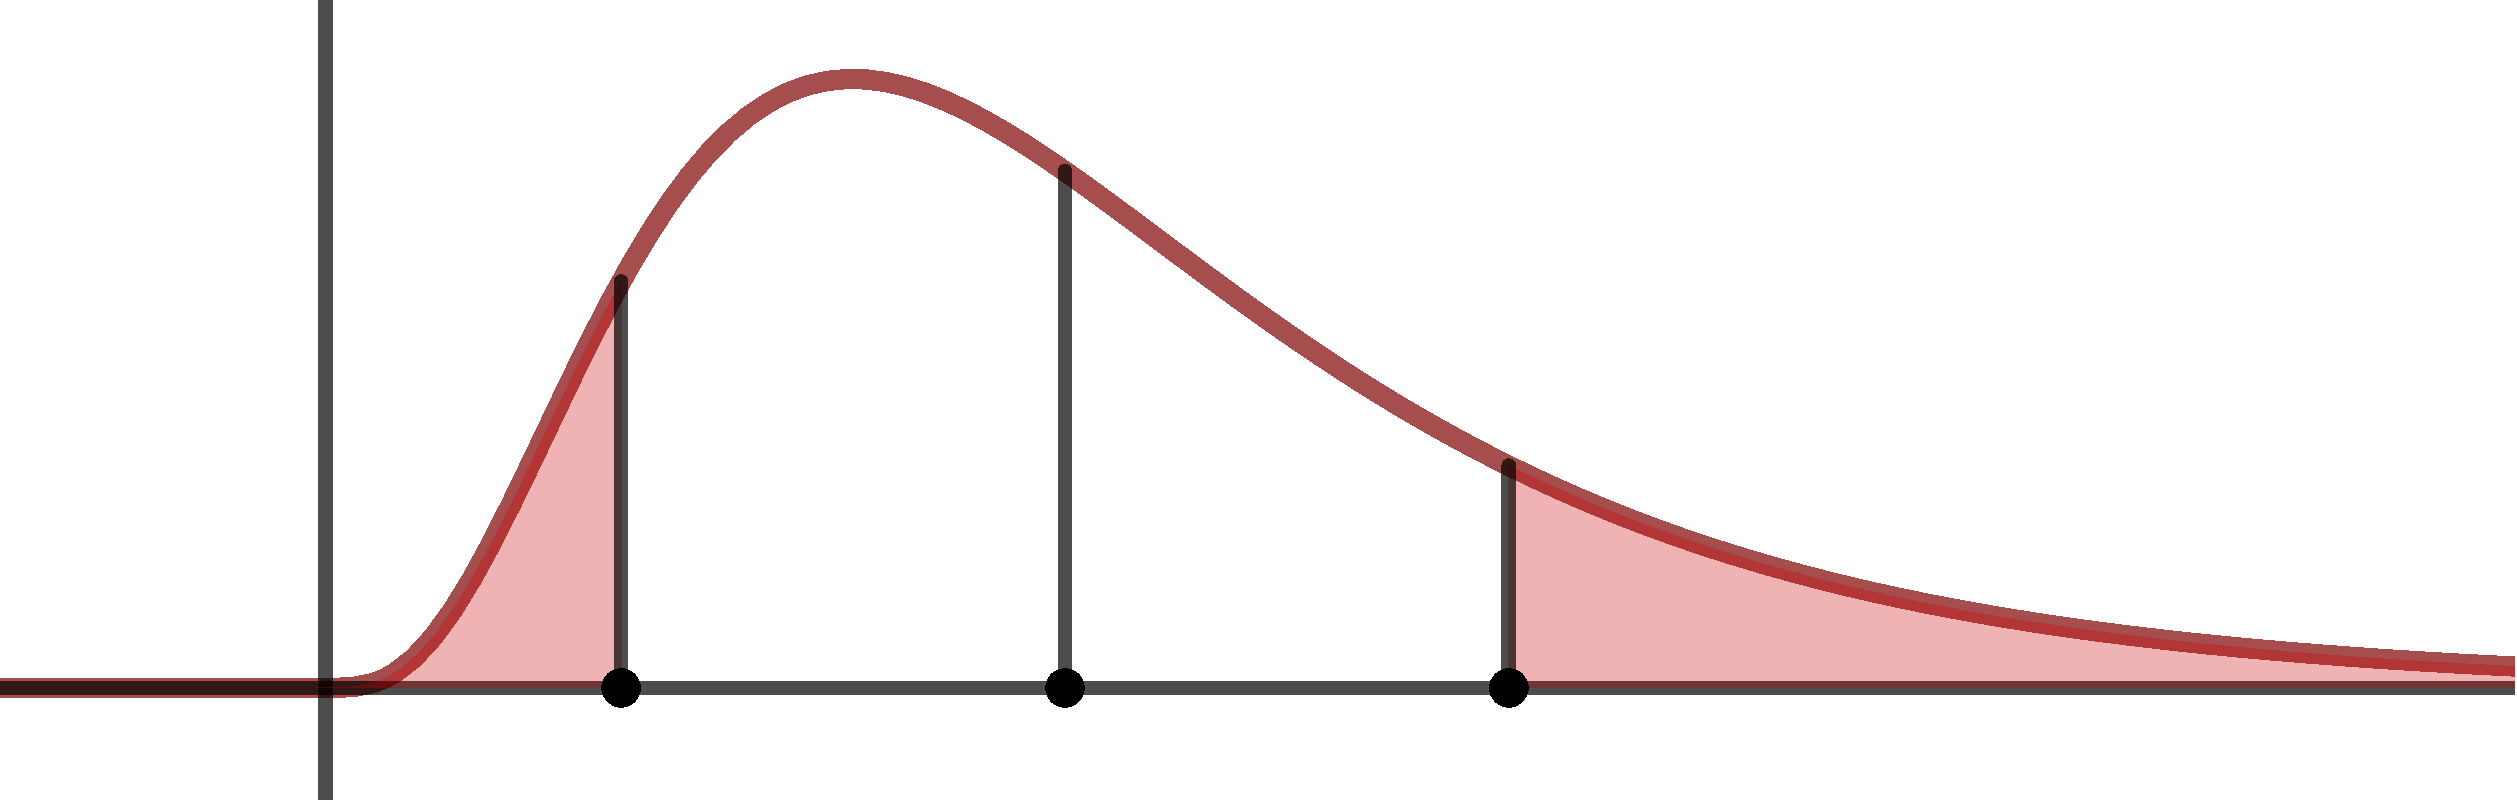
\includegraphics[width=10cm]{Images/FDistrib}};
	\draw [color=black](-3.1,-0.45) node[anchor=north west] {$\frac{\alpha}{2}$};
	\draw [color=black](1.0,-0.45) node[anchor=north west] {$\frac{\alpha}{2}$};
	\draw [color=red!20!black](0.35,1.00) node[anchor=north west] {Fisherova distribuce};
	\draw [color=red!40!black](0.7,0.50) node[anchor=north west] {$F_{12}\sim\FF(n_1-1,n_2-1)$};
	\draw [color=black](-4.2,-1.25) node[anchor=north west] {$0$};
	\draw [color=black](-2.9,-1.25) node[anchor=north west] {$K_L$};
	\draw [color=black](-1,-1.25) node[anchor=north west] {$1$};
	\draw [color=black](0.75,-1.25) node[anchor=north west] {$K_H$};
	\end{tikzpicture}
	\caption{Kritický obor F-testu homogenity rozptylů.}
	\label{fig:fisher}
\end{figure}
\begin{remark}
		V praxi lze použít testovací statistiku $$\widetilde{F}_{12}=\frac{\max(s_1^2,s_2^2)}{\min(s_1^2,s_2^2)}\sim \FF(n'-1,n''-1),\text{ kde }\quad \begin{array}{l}
	n'= \max(n_1,n_2),\\n''=\min(n_1,n_2),
	\end{array} $$ kterou pak porovnáváme pouze s~horním $\FF_{1-\frac{\alpha}{2}}$ příslušným kvantilem Fisherova rozdělení.
\end{remark}
\section{Test koeficientu korelace ($\mathcal{N}_2$)}
Předpokládejme $ (X_j,Y_j)_{j=1}^n ~iid~\NN_2(\mu_1,\mu_2,\sigma_1^2,\sigma_2^2,\rho)$ z~dvourozměrného nedegenerovaného Gaussova rozdělení při~$\sigma_1>0,~\sigma_2>0,~\abs{\rho}<1$. Testujeme nekorelovanost $X,Y$, tzn. nulovou hodnotu korelačního koeficientu $\rho=\rho(X,Y)$: $$H_0:\rho=0~\text{vs.}~H_1:\rho\neq 0\qquad(\text{tzn. test nezávislosti }X\text{ a~}Y\text{ v~}\NN_2\text{ modelu})$$ na~hladině významnosti $\alpha\in(0,1)$.\\
\textbf{Odvodíme LRT test} $H_0$:\\
Logaritmická věrohodnostní funkce modelu $\NN_2(\mu_1,\mu_2,\sigma_1^2,\sigma_2^2,\rho)$ při~označení $\t=(\mu_1,\mu_2,\sigma_1^2,\sigma_2^2,\rho)$ je 
\[
\begin{split}
&l(\t)=\ln L(\t)=\frac{-1}{2(1-\rho^2)}\Big[ \sum\limits_{j=1}^{n}\frac{(X_j-\mu_1)^2}{\sigma_1^2}+\sum\limits_{j=1}^{n}\frac{(Y_j-\mu_2)^2}{\sigma_2^2}-\\&-2\rho\sum\limits_{j=1}^{n}\frac{(X_j-\mu_1)(Y_j-\mu_2)}{\sigma_1\sigma_2}\Big] -n\ln\br{2\pi\sigma_1\sigma_2\sqrt{1-\rho^2}} . \end{split}
\]
Následně vyhodnotíme výraz
$$ \Lambda(\textbf{x},\textbf{y})=\frac{\sup\{ L(\t):\mu_1,\mu_2,\sigma_1^2,\sigma_2^2,\rho=0 \}}{\sup\{ L(\t):\mu_1,\mu_2,\sigma_1^2,\sigma_2^2,|\rho|<1\}}\sim \frac{\text{4 rovnice typu }\partial_r \ln L=0}{\text{5 rovnic typu }\partial_l\ln L=0}.$$
Řešením obou extrémů jsou MLE odhady: $\widehat{\mu}_1=\oxn$, $\widehat{\mu}_2=\oyn$, $\widehat{\sigma}_1^2=\widehat{\sigma}_{n,X}^2$ a~$\widehat{\sigma}_2^2=\widehat{\sigma}_{n,Y}^2$ a~dále
$$ \widehat{\rho}_{_{XY}}=\widehat{\rho}_{n}(\X,\Y)=\frac{\sum_{j=1}^n (X_j-\Oxn)(Y_j-\Oyn)}{\sqrt{\sum_{j=1}^n(X_j-\Oxn)^2\sum_{j=1}^n(Y_j-\Oyn)^2}}=\frac{\widehat{\Cov}_{XY}}{\widehat{\sigma}_1\cdot\widehat{\sigma}_2}, $$ který se~nazývá \textbf{Pearsonův výběrový koeficient korelace}. Dosazením těchto odhadů do~$\Lambda(\textbf{x},\textbf{y})$ získáme 
\[
\begin{split}
\ln\Lambda(\textbf{x},\textbf{y})&=\ln L(\widehat{\mu}_1,\widehat{\mu}_2,\widehat{\sigma}_1,\widehat{\sigma}_2,\rho=0)-\ln L(\widehat{\mu}_1,\widehat{\mu}_2,\widehat{\sigma}_1,\widehat{\sigma}_2,\widehat{\rho}_{XY})=\\&=-n\ln(2\pi\widehat{\sigma}_1\widehat{\sigma}_2)+n\ln\br{2\pi \widehat{\sigma}_1\widehat{\sigma}_2\sqrt{1-\widehat{\rho}_{XY}^2}}=\\&=\frac{n}{2}\ln\br{1-\widehat{\rho}_{XY}^2}\leq K~\Leftrightarrow~ \big| \widehat{\rho}_{XY} \big|\geq K'\Leftrightarrow~ \frac{|\widehat{\rho}_{XY}|\sqrt{n-2}}{\sqrt{1-\widehat{\rho}_{XY}^2}}\geq K'',
\end{split}
\]
kde $K,K',K''$ jsou vhodné konstanty nezávislé na~$(\textbf{x},\textbf{y})$. Lze ukázat, že při~platnosti $H_0:\rho=0$ má testovací LRT statistika rozdělení $$T=T(\X,\Y)=\frac{\widehat{\rho}_{_{XY}}\sqrt{n-2}}{\sqrt{1-\widehat{\rho}_{_{XY}}^2}}\sim t(n-2),$$ tedy Studentovo rozdělení s~$(n-2)$ stupni volnosti. To vede na~kritický obor testu $H_0:\rho=0$ ve~tvaru $$ W_\alpha=\left\{ (\textbf{x},\textbf{y}):\abs{T(\textbf{x},\textbf{y})}\geq t_{1-\frac{\alpha}{2}}(n-2) \right\}, $$ opět s~použitím $\Br{1-\frac{\alpha}{2}}$-kvantilu příslušného Studentova rozdělení.
\begin{example} Mějme následující dvourozměrná pozorování (data) o~rozsahu $n=10$
	$$	\begin{array}{c|cccccccccc}
	x_j & 94 & 98 & 127 & 88 & 85 & 95 & 111 & 75 & 102 & 82 \\ \hline
	y_j & 2.1 & 1.9 & 3.5 & 1.5 & 3.2 & 1.6 & 1.9 & 2.5 & 2.6 & 1.9
	\end{array} $$ pocházející z~náhodného výběru $(X_j,Y_j)_{j=1}^n~iid~\NN(\mu_1,\mu_2,\sigma_1^2,\sigma_2^2,\rho)$. Pro~test nekorelovanosti (zde i~test nezávislosti) $X$ a~$Y$ na~hladině $\alpha=0.05$ spočteme pro~$n=10$ následující hodnoty $$
	\widehat{\rho}_{X,Y}=0.3425,\quad T=\frac{\widehat{\rho}_{XY}\sqrt{n-2}}{\sqrt{1-\widehat{\rho}_{XY}^2}}=1.031,\quad
	t_{1-\alpha/2}(n-2)=t_{0.975}(8)=2.306.$$
	Nyní tedy testujeme $W_\alpha:~|T|\geq t_{0.975}(8)$? Nerovnost ale neplatí, a~proto $H_0$ nezamítáme na~hladině $\alpha=0.05$.
	Pokud síla testu $\beta$ (silofunkce) je dostatečně vysoká, např. $\beta>\beta_1$ na intervalu $\rho\in(-1,-\delta)\cup(\delta,1)$, pak $H_0$ přijímáme, tzn. s~danou signifikací $1-\beta_1$ deklarujeme, že mezi~Gaussovskými náhodnými veličinami $X$ a~$Y$ není korelační vztah, tedy $X$ a~$Y$ jsou nezávislé.
\end{example}
